\documentclass[10pt]{beamer}

\setbeamertemplate{footline}[page number]

\usepackage{tikz}

\title{Computing Euler factors}
\subtitle{Study group on models of curves and arithmetic applications}
\author{David Kurniadi Angdinata}
\institute{London School of Geometry and Number Theory}
\date{Wednesday, 2 April 2025}

\begin{document}

\frame{\titlepage}

\begin{frame}{Notation}

\begin{itemize}
\item[$ p $] an odd prime (of almost good reduction)
\item[$ C $] a smooth projective (hyperelliptic) curve of genus $ g $ ($ = 2 $) over $ \mathbb{Q} $ (with semistable reduction at $ p $) given by an integral model
$$ Y^2 = c\prod_{r \in \mathcal{R}} (X - r), \qquad c \in \mathbb{Z}, \qquad r \in \overline{\mathbb{Q}}. $$
\item[$ \mathcal{C} $] the minimal regular model of $ C $ at $ p $
\item[$ \widetilde{\mathcal{C}} $] the special fibre of $ \mathcal{C} $
\item[$ \overline{C} $] the base change of $ C $ to $ \overline{\mathbb{Q}} $
\item[$ \overline{\widetilde{\mathcal{C}}} $] the base change of $ \widetilde{\mathcal{C}} $ to $ \overline{\mathbb{F}_p} $
\end{itemize}

\end{frame}

\begin{frame}[t]{L-functions}

Recall that the L-function of $ C $ is the Euler product
$$ L(C, s) := \prod_p \dfrac{1}{L_p(C, p^{-s})}, $$
over all primes $ p $, where the local Euler factor at $ p $ is the polynomial
$$ L_p(C, T) := \det(1 - T \cdot \operatorname{Frob}_p^{-1} \mid H_{\text{\'et}}^1(\overline{C}, \mathbb{Q}_\ell)^{I_p}). $$
When $ C $ has semistable reduction at $ p $,
$$ H_{\text{\'et}}^1(\overline{C}, \mathbb{Q}_\ell)^{I_p} \cong H_{\text{\'et}}^1(\overline{\widetilde{\mathcal{C}}}, \mathbb{Q}_\ell), $$
which is an isomorphism of $ \operatorname{Gal}(\overline{\mathbb{Q}_p} / \mathbb{Q}_p) $-representations, so that
$$ L_p(C, T) = \det(1 - T \cdot \operatorname{Frob}_p^{-1} \mid H_{\text{\'et}}^1(\overline{\widetilde{\mathcal{C}}}, \mathbb{Q}_\ell)). $$
This can be extracted from the $ \zeta $-function of $ \widetilde{\mathcal{C}} $.

\end{frame}

\begin{frame}[t]{$ \zeta $-functions}

The $ \zeta $-function of a projective curve $ X $ over $ \mathbb{F}_p $ is the rational function
$$ \zeta(X, T) := \exp\left(\sum_{k \ge 1} \#X(\mathbb{F}_{p^k})\dfrac{T^k}{k}\right) = \dfrac{P_1(X, T)}{P_0(X, T) \cdot P_2(X, T)}, $$
by the Weil conjectures, where
$$ P_i(X, T) := \det(1 - T \cdot \operatorname{Frob}_p^{-1} \mid H_{\text{\'et}}^1(X, \mathbb{Q}_\ell)), \qquad i = 0, 1, 2. $$
When the Jacobian $ \operatorname{Jac}(C) $ of $ C $ has good reduction at $ p $,
$$ P_0(\widetilde{\mathcal{C}}, T) = 1 - T, \qquad \deg P_1(\widetilde{\mathcal{C}}, T) = 2g, \qquad P_2(\widetilde{\mathcal{C}}, T) = 1 - pT, $$
so that $ L_p(C, T) $ is determined by $ \#\widetilde{\mathcal{C}}(\mathbb{F}_{p^k}) $ for sufficiently many $ k \ge 1 $.

\vspace{0.5cm} In general, this requires computing the minimal regular model $ \mathcal{C} $ by a resolution of singularities, which is computationally expensive.

\end{frame}

\begin{frame}[t]{Cluster pictures}

Instead of computing $ \mathcal{C} $, its special fibre $ \widetilde{\mathcal{C}} $ can be recovered from cluster picture machinery, with explicit models for its irreducible components.

\vspace{0.5cm} Recall that a cluster is a non-empty subset of $ \mathcal{R} $ of the form
$$ \mathfrak{s} = \{r \in \mathcal{R} \mid \nu_p(r - z) \ge d\}, \qquad z \in \overline{\mathbb{Q}_p}, \qquad d \in \mathbb{Q}. $$
The depth $ d_\mathfrak{s} $ of a cluster $ \mathfrak{s} $ is the largest such $ d $, in which case any $ z $ with $ \nu_p(r - z) = d_\mathfrak{s} $ for some $ r \in \mathfrak{s} $ is called a centre $ z_\mathfrak{s} $ of $ \mathfrak{s} $. A child of $ \mathfrak{s} $ is a maximal subcluster $ \mathfrak{s}' \subsetneq \mathfrak{s} $, and its relative depth $ \delta_{\mathfrak{s}'} $ is simply $ d_{\mathfrak{s}'} - d_\mathfrak{s} $.

\vspace{0.5cm} A cluster $ \mathfrak{s} $ is called odd or even if $ |\mathfrak{s}| $ is odd or even respectively. It is called \"ubereven if every child of $ \mathfrak{s} $ is even. It is called twin if $ |\mathfrak{s}| = 2 $, and it is called cotwin if it is not \"ubereven but it has a child $ \mathfrak{s}' $ with $ |\mathfrak{s}'| = 2g $.

\vspace{0.5cm} The cluster $ \mathcal{R} $ is called principal if it is odd or if it has more than two children. In general, a cluster $ \mathfrak{s} $ is called principal when $ |\mathfrak{s}| \ge 3 $ but has no children $ \mathfrak{s}' $ with $ |\mathfrak{s}'| = 2g $.

\end{frame}

\begin{frame}[t]{Cluster picture example}

Let $ C $ be the hyperelliptic curve over $ \mathbb{Q} $ given by
$$ Y^2 = 2X(X - 1)(X - p^n)(X - 2p^n)(X - p^m)(X - 2p^m), $$
where $ p $ is an odd prime and $ m \ge n $ are positive integers.

\vspace{0.5cm} The associated cluster picture is:
$$
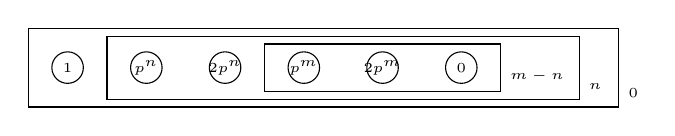
\begin{tikzpicture}
\draw (0, 0) rectangle (7.5, -1) node[above right]{\tiny $ 0 $};
\draw (0.5, -0.5) circle (0.2) node{\tiny $ 1 $};
\draw (1, -0.1) rectangle (7, -0.9) node[above right]{\tiny $ n $};
\draw (1.5, -0.5) circle (0.2) node{\tiny $ p^n $};
\draw (2.5, -0.5) circle (0.2) node{\tiny $ 2p^n $};
\draw (3, -0.2) rectangle (6, -0.8) node[above right]{\tiny $ m - n $};
\draw (3.5, -0.5) circle (0.2) node{\tiny $ p^m $};
\draw (4.5, -0.5) circle (0.2) node{\tiny $ 2p^m $};
\draw (5.5, -0.5) circle (0.2) node{\tiny $ 0 $};
\end{tikzpicture}
$$

The cluster $ \mathcal{R} $ is not principal, but it has two principal subclusters.
\begin{itemize}
\item The odd subcluster $ \mathfrak{s}_m := \{p^m, 2p^m, 0\} $ has centre $ z_{\mathfrak{s}_m} = 0 $, depth $ d_{\mathfrak{s}_m} = m $ and relative depth $ \delta_{\mathfrak{s}_m} = m - n $.
\item The odd subcluster $ \mathfrak{s}_n := \{p^n, 2p^n, p^m, 2p^m, 0\} $ has centre $ z_{\mathfrak{s}_n} = p^n $, depth $ d_{\mathfrak{s}_n} = n $, and relative depth $ \delta_{\mathfrak{s}_n} = n $.
\end{itemize}
Neither subclusters are \"ubereven or cotwin.

\end{frame}

\begin{frame}[t]{Components of special fibres}

\begin{theorem}[M2D2, Theorem 8.6(1)]
Let $ C $ be a hyperelliptic curve over $ \mathbb{Q} $ given by
$$ Y^2 = c\prod_{r \in \mathcal{R}} (X - r), \qquad c \in \mathbb{Z}, \qquad r \in \overline{\mathbb{Q}}. $$
Assume that $ C $ has semistable reduction at some odd prime $ p $, and that $ \delta_\mathfrak{s} \ne \tfrac{1}{2} $ for any principal cluster $ \mathfrak{s} $. Then the components of $ \widetilde{\mathcal{C}} $ consist of the curves $ \Gamma_\mathfrak{s} $ associated to principal clusters $ \mathfrak{s} $, given by
$$ Y^2 = \widetilde{\dfrac{c}{p^{\nu_p(c)}}}\prod_{r \in \mathcal{R} \setminus \mathfrak{s}} \widetilde{\dfrac{z_\mathfrak{s} - r}{p^{\nu_p(z_\mathfrak{s} - r)}}}\prod_{\text{odd} \ \mathfrak{s}' < \mathfrak{s}} \left(X - \widetilde{\dfrac{z_{\mathfrak{s}'} - z_\mathfrak{s}}{p^{d_\mathfrak{s}}}}\right). $$
This is irreducible except when $ \mathfrak{s} $ is \"ubereven, in which case it has two irreducible components $ \Gamma_\mathfrak{s}^+ $ and $ \Gamma_\mathfrak{s}^- $. The remaining components of $ \widetilde{\mathcal{C}} $ are chains of $ \mathbb{P}^1 $ that link $ \Gamma_\mathfrak{s} $, which are given by the following conditions.
\end{theorem}

\end{frame}

\begin{frame}[t]{Intersections of special fibres}

\begin{theorem}[M2D2, Theorem 8.6(1), continued]
\begin{itemize}
\item Assume that $ \mathfrak{s}' < \mathfrak{s} $.
\begin{itemize}
\item When $ \mathfrak{s}' $ is principal odd and $ \mathfrak{s} $ is principal, then there is a chain from $ \Gamma_{\mathfrak{s}'} $ to $ \Gamma_\mathfrak{s} $ of length $ \tfrac{1}{2}\delta_{\mathfrak{s}'} - 1 $.
\item When $ \mathfrak{s}' $ is principal even and $ \mathfrak{s} $ is principal, then there are two chains from $ \Gamma_{\mathfrak{s}'}^+ $ to $ \Gamma_\mathfrak{s}^+ $ and from $ \Gamma_{\mathfrak{s}'}^- $ to $ \Gamma_\mathfrak{s}^- $ each of length $ \delta_{\mathfrak{s}'} - 1 $.
\item When $ \mathfrak{s}' $ is twin and $ \mathfrak{s} $ is principal, then there is a chain from $ \Gamma_\mathfrak{s}^- $ to $ \Gamma_\mathfrak{s}^+ $ of length $ 2\delta_{\mathfrak{s}'} - 1 $.
\item When $ \mathfrak{s}' $ is principal and $ \mathfrak{s} $ is cotwin, then there is a chain from $ \Gamma_{\mathfrak{s}'}^- $ to $ \Gamma_{\mathfrak{s}'}^+ $ of length $ 2\delta_{\mathfrak{s}'} - 1 $.
\end{itemize}
\item Assume that $ \mathcal{R} $ is not principal, but $ \mathcal{R} = \mathfrak{s}_1 \sqcup \mathfrak{s}_2 $.
\begin{itemize}
\item When $ \mathfrak{s}_1 $ and $ \mathfrak{s}_2 $ are principal odd, then there is a chain from $ \Gamma_{\mathfrak{s}_1} $ to $ \Gamma_{\mathfrak{s}_2} $ of length $ \tfrac{1}{2}(\delta_{\mathfrak{s}_1} + \delta_{\mathfrak{s}_2}) - 1 $.
\item When $ \mathfrak{s}_1 $ and $ \mathfrak{s}_2 $ are principal even, then there are two chains from $ \Gamma_{\mathfrak{s}_1}^+ $ to $ \Gamma_{\mathfrak{s}_2}^+ $ and from $ \Gamma_{\mathfrak{s}_1}^- $ to $ \Gamma_{\mathfrak{s}_2}^- $ each of length $ \delta_{\mathfrak{s}_1} + \delta_{\mathfrak{s}_2} - 1 $.
\item When $ \mathfrak{s}_1 $ is principal even and $ \mathfrak{s}_2 $ is twin, then there is a chain from $ \Gamma_{\mathfrak{s}_1}^- $ to $ \Gamma_{\mathfrak{s}_1}^+ $ of length $ 2(\delta_{\mathfrak{s}_1} + \delta_{\mathfrak{s}_2}) - 1 $.
\end{itemize}
\end{itemize}
\end{theorem}

\end{frame}

\begin{frame}[t]{Special fibre example}

Continuing on the previous example, $ \Gamma_{\mathfrak{s}_m} $ computes to be
\begin{align*}
Y^2 & = 2\widetilde{\left(\dfrac{0 - 1}{p^{\nu_p(0 - 1)}}\right)}\widetilde{\left(\dfrac{0 - p^n}{p^{\nu_p(0 - p^n)}}\right)}\widetilde{\left(\dfrac{0 - 2p^n}{p^{\nu_p(0 - 2p^n)}}\right)} \\
& \qquad \left(X - \widetilde{\dfrac{p^m - 0}{p^m}}\right)\left(X - \widetilde{\dfrac{2p^m - 0}{p^m}}\right)\left(X - \widetilde{\dfrac{0 - 0}{p^m}}\right) \\
& = -4X(X - 1)(X - 2),
\end{align*}
and $ \Gamma_{\mathfrak{s}_n} $ computes to be
\begin{align*}
Y^2 & = 2\widetilde{\left(\dfrac{p^n - 1}{p^{\nu_p(p^n - 1)}}\right)}\left(X - \widetilde{\dfrac{p^n - p^n}{p^n}}\right)\left(X - \widetilde{\dfrac{2p^n - p^n}{p^n}}\right)\left(X - \widetilde{\dfrac{0 - p^n}{p^n}}\right) \\
& = -2X(X - 1)(X + 1).
\end{align*}
Furthermore, there is a chain from $ \Gamma_{\mathfrak{s}_m} $ to $ \Gamma_{\mathfrak{s}_n} $ of length $ \tfrac{1}{2}(m - n) - 1 $.

\end{frame}

\begin{frame}[t]{$ \zeta $-function example}

Recall that to compute $ \zeta(\widetilde{\mathcal{C}}, T) $, it suffices to compute
$$ \#C(\mathbb{F}_{p^k}) = \#\Gamma_{\mathfrak{s}_m}(\mathbb{F}_{p^k}) + \#\Gamma_{\mathfrak{s}_n}(\mathbb{F}_{p^k}) + \left(\dfrac{m - n}{2} - 1\right)\#\mathbb{P}^1(\mathbb{F}_{p^k}) - \dfrac{m - n}{2}, $$
for all $ k \ge 1 $. For instance, if $ p = 5 $, then
\begin{align*}
\#\Gamma_{\mathfrak{s}_m}(\mathbb{F}_{5^k}) & = 1 - ((-1 - 2i)^k + (-1 + 2i)^k) + 5^k, \\
\#\Gamma_{\mathfrak{s}_n}(\mathbb{F}_{5^k}) & = 1 - ((1 - 2i)^k + (1 + 2i)^k) + 5^k,
\end{align*}
and if $ m = 16 $ and $ n = 10 $, then
$$ \#C(\mathbb{F}_{5^k}) = 1 + 4 \cdot 5^k - \sum_\pm (\pm1 \pm 2i)^k, $$
so that
$$ \zeta(\widetilde{\mathcal{C}}, T) = \dfrac{\prod_\pm (1 - (\pm1 \pm 2i)T)}{(1 - T)(1 - 5T)^4} = \dfrac{(1 - 2T + 5T^2)(1 + 2T + 5T^2)}{(1 - T)(1 - 5T)^4}. $$

\end{frame}

\begin{frame}[t]{Almost good primes}

Unlike elliptic curves, there are higher genus curves $ C $ over $ \mathbb{Q} $ with primes $ p $ that divide its minimal discriminant $ \Delta_C $ but do not divide its conductor $ \mathfrak{f}_C $, such as when $ \operatorname{Jac}(C) $ reduces to a product of elliptic curves over $ \mathbb{F}_p $. These primes $ p $ are called primes of \textbf{almost good reduction} for $ C $.

\vspace{0.5cm} For instance, the genus two curve over $ \mathbb{Q} $ given by
\begin{align*}
& Y^2 + (X^3 + X^2 + X)Y = -144061786290072X^6 - 23062462482396X^5 \\
& \qquad - 1266273619292236X^4 - 3052943051575761X^3 \\
& \qquad + 3989955132045666X^2 + 3438312415pX - 1707513566p
\end{align*}
has $ \mathfrak{f}_C = 270761 $ but $ \Delta_C = 270761p^{22} $ where $ p = 14556001 $.

\vspace{0.5cm} Maistret and Sutherland were motivated to expand the LMFDB, which currently contains $ 66158 $ genus two curves $ C $ over $ \mathbb{Q} $ with $ \Delta_C \le 10^6 $, to over $ 5 \cdot 10^6 $ genus two curves $ C $ over $ \mathbb{Q} $ with $ \mathfrak{f}_C \le 2^{20} \approx 10^6 $.

\end{frame}

\begin{frame}[t]{Cluster pictures at almost good primes}

The prime of almost good reduction forces the existence of a subcluster of size $ 3 $, all subclusters to be odd, and specific conditions on their depths.

\begin{theorem}[MS25, Corollaries 3.5/7/10/11]
Let $ C $ be a hyperelliptic curve over $ \mathbb{Q} $ given by $ Y^2 = \sum_{i = 0}^6 c_iX^i \in \mathbb{Z}[X] $ such that $ d_\mathcal{R} = 0 $ and $ \nu_p(c_6) = \min_i\nu_p(c_i) \le 1 $ at some odd prime $ p $ of almost good reduction. Then its cluster picture is one of the following:
\begin{align*}
&
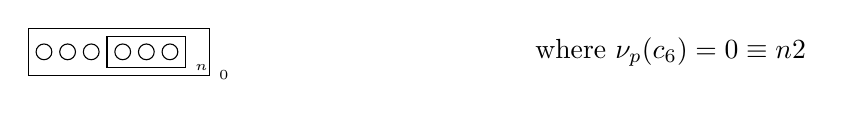
\begin{tikzpicture}
\draw (0, 0) rectangle (2.3, -0.6) node[right]{\tiny $ 0 $};
\draw (0.2, -0.3) circle (0.1);
\draw (0.5, -0.3) circle (0.1);
\draw (0.8, -0.3) circle (0.1);
\draw (1, -0.1) rectangle (2, -0.5) node[right]{\tiny $ n $};
\draw (1.2, -0.3) circle (0.1);
\draw (1.5, -0.3) circle (0.1);
\draw (1.8, -0.3) circle (0.1);
\draw (10, -0.3) node[left]{where $ \nu_p(c_6) = 0 \equiv n \mod 2 $};
\end{tikzpicture}
\\ &
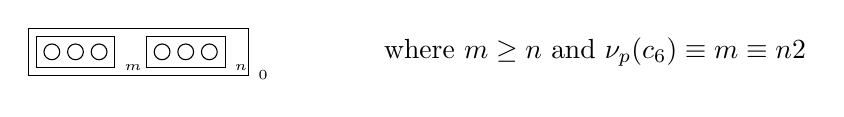
\begin{tikzpicture}
\draw (0, 0) rectangle (2.8, -0.6) node[right]{\tiny $ 0 $};
\draw (0.1, -0.1) rectangle (1.1, -0.5) node[right]{\tiny $ m $};
\draw (0.3, -0.3) circle (0.1);
\draw (0.6, -0.3) circle (0.1);
\draw (0.9, -0.3) circle (0.1);
\draw (1.5, -0.1) rectangle (2.5, -0.5) node[right]{\tiny $ n $};
\draw (1.7, -0.3) circle (0.1);
\draw (2, -0.3) circle (0.1);
\draw (2.3, -0.3) circle (0.1);
\draw (10, -0.3) node[left]{where $ m \ge n $ and $ \nu_p(c_6) \equiv m \equiv n \mod 2 $};
\end{tikzpicture}
\\ &
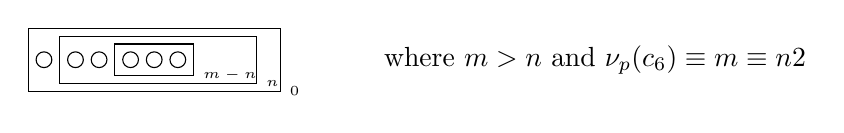
\begin{tikzpicture}
\draw (0, 0) rectangle (3.2, -0.8) node[right]{\tiny $ 0 $};
\draw (0.2, -0.4) circle (0.1);
\draw (0.4, -0.1) rectangle (2.9, -0.7) node[right]{\tiny $ n $};
\draw (0.6, -0.4) circle (0.1);
\draw (0.9, -0.4) circle (0.1);
\draw (1.1, -0.2) rectangle (2.1, -0.6) node[right]{\tiny $ m - n $};
\draw (1.3, -0.4) circle (0.1);
\draw (1.6, -0.4) circle (0.1);
\draw (1.9, -0.4) circle (0.1);
\draw (10, -0.4) node[left]{where $ m > n $ and $ \nu_p(c_6) \equiv m \equiv n \mod 2 $};
\end{tikzpicture}
\end{align*}
Furthermore, there is an explicit description for $ \widetilde{\mathcal{C}} $ as the union of two elliptic curves over $ \mathbb{F}_{p^2} $ linked by a chain of $ \mathbb{P}^1 $ for each cluster picture.
\end{theorem}

\end{frame}

\begin{frame}[t]{Computing Euler factors}

It turns out that any genus two curve over $ \mathbb{Q} $ with almost good reduction at an odd prime can be normalised to obtain such a model.

\begin{theorem}[MS25, Theorem 1.1]
Let $ C $ be a genus two curve over $ \mathbb{Q} $ given by $ Y^2 = \sum_{i = 0}^6 c_iX^i \in \mathbb{Z}[X] $ with almost good reduction at some odd prime $ p $. Then there is a probabilistic algorithm that computes $ L_p(C, T) $ with running time
$$ O\left(\dfrac{(\max_i\log|c_i|)^2\log^2(\max_i\log|c_i|)}{\log p} + \log^5p\right). $$
Furthermore, if a quadratic non-residue modulo $ p $ is given, then the algorithm is deterministic with the same running time.
\end{theorem}

\vspace{0.5cm} This has been implemented in Magma in the public \texttt{Genus2Euler} repository. In a test on $ 3454506 $ pairs of $ (C, p) $, it is almost $ 5000 $ times faster than the existing \texttt{EulerFactor} function in Magma, including $ 489 $ pairs of $ (C, p) $ whose computations were terminated after eight hours.

\end{frame}

\begin{frame}{References}

\begin{itemize}
\item[MS25] C\'eline Maistret, Andrew Sutherland. Computing Euler factors of genus 2 curves at odd primes of almost good reduction. Research in Number Theory 11, 37 (2025). https://doi.org/10.1007/s40993-024-00605-7
\item[M2D2] Tim Dokchitser, Vladimir Dokchitser, C\'eline Maistret, Adam Morgan. Arithmetic of hyperelliptic curves over local fields. Mathematische Annalen 385, 1213-1322 (2023). https://doi.org/10.1007/s00208-021-02319-y
\end{itemize}

\end{frame}

\end{document}